\documentclass[11pt]{article}
\usepackage[textwidth=18.0cm, textheight=23.0cm, top=2.0cm]{geometry}
\usepackage{pst-all}
\usepackage{amssymb}
\usepackage{tikz}
\usepackage{underscore}\begin{document}
\pagestyle{empty}


ClassName: \underline{\textbf{Class_10.2bp-26}}
\par
BinSize: \underline{\textbf{100 × 100}}
\par
ReduceSize: \underline{\textbf{100 × 100}}
\par
TypeNum: \underline{\textbf{60}}
\par
Num: \underline{\textbf{60}}
\par
OutS: \underline{\textbf{100000}}
\par
InS: \underline{\textbf{89755}}
\par
Rate: \underline{\textbf{0.898}}
\par
UB: \underline{\textbf{10}}
\par
LB0: \underline{\textbf{10}}
\par
LB: \underline{\textbf{10}}
\par
LBWithCut: \underline{\textbf{10}}
\par
NodeCut: \underline{\textbf{0}}
\par
ExtendedNodeCnt: \underline{\textbf{1}}
\par
GenNodeCnt: \underline{\textbf{1}}
\par
PrimalNode: \underline{\textbf{0}}
\par
ColumnCount: \underline{\textbf{10}}
\par
TotalCutCount: \underline{\textbf{0}}
\par
RootCutCount: \underline{\textbf{0}}
\par
LPSolverCnt: \underline{\textbf{1}}
\par
PricingSolverCnt: \underline{\textbf{0}}
\par
BranchAndBoundNum: \underline{\textbf{1}}
\par
isOpt: \underline{\textbf{true}}
\par
TimeOnInitSolution: \underline{\textbf{600.000 s}}
\par
TimeOnPrimal: \underline{\textbf{0.000 s}}
\par
TimeOnPricing: \underline{\textbf{0.000 s}}
\par
TimeOnRmp: \underline{\textbf{0.058 s}}
\par
TotalTime: \underline{\textbf{600.302 s}}
\par
\newpage


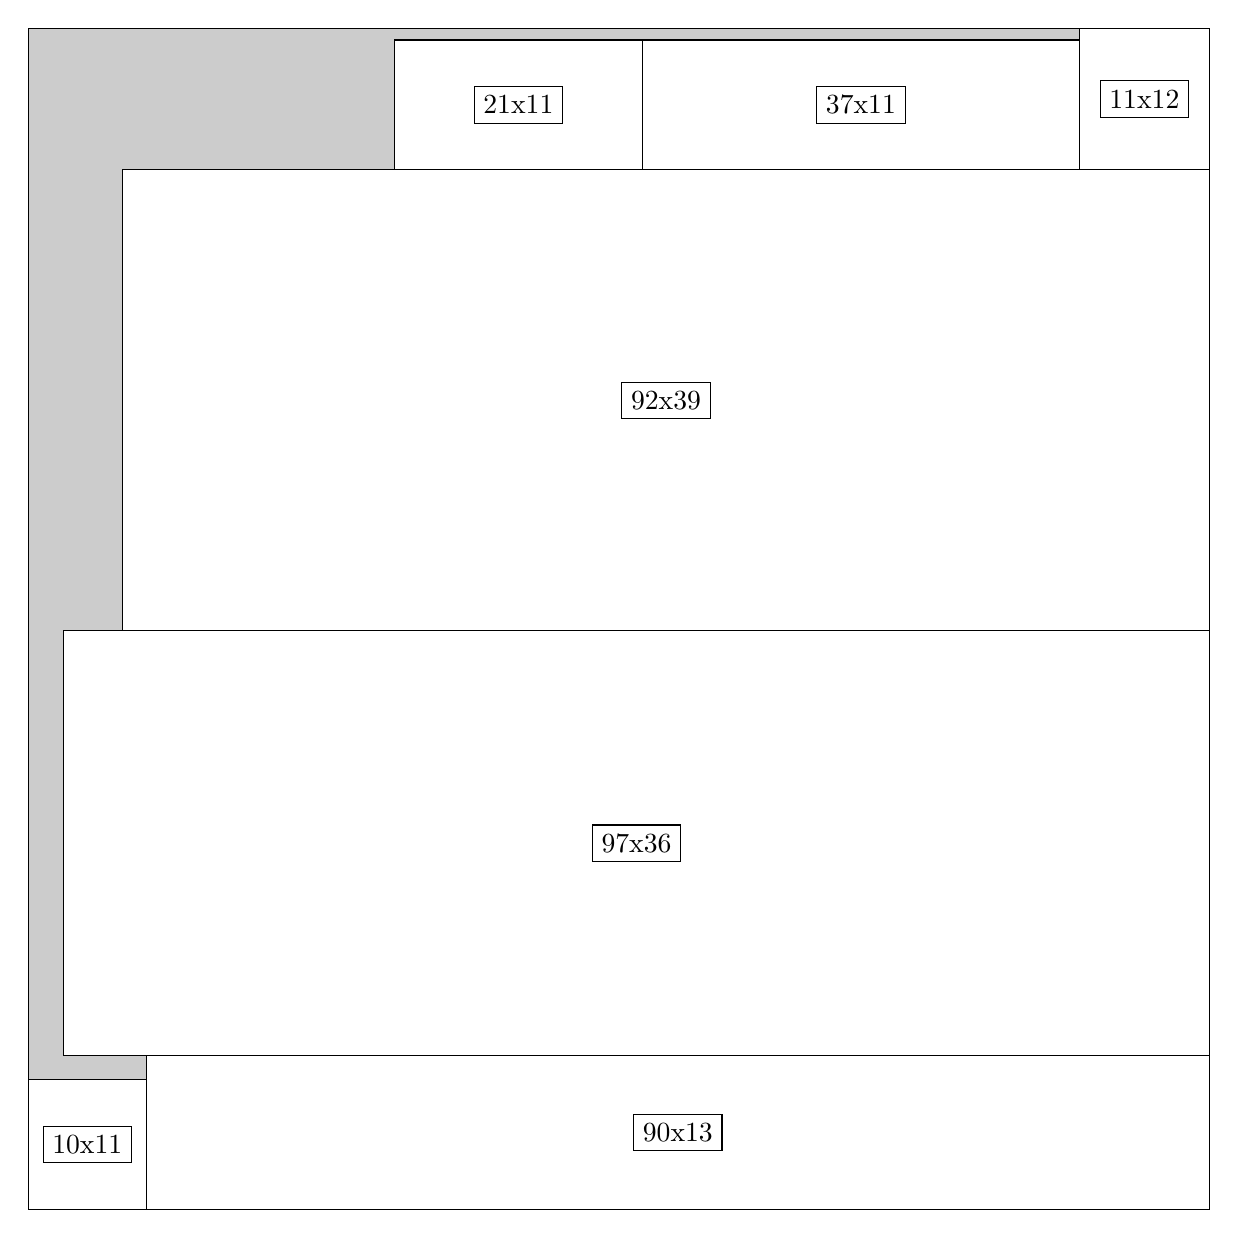
\begin{tikzpicture}[shorten >=1pt,scale=1.0,every node/.style={scale=1.0},->]
\tikzstyle{vertex}=[circle,fill=black!25,minimum size=14pt,inner sep=0pt]
\filldraw[fill=gray!40!white, draw=black] (0,0) rectangle (15.0,15.0);
\foreach \name/\x/\y/\w/\h in {90x13/1.5/0.0/13.5/1.95,10x11/0.0/0.0/1.5/1.65,97x36/0.44999999999999996/1.95/14.549999999999999/5.3999999999999995,92x39/1.2/7.35/13.799999999999999/5.85,11x12/13.35/13.2/1.65/1.7999999999999998,37x11/7.8/13.2/5.55/1.65,21x11/4.6499999999999995/13.2/3.15/1.65}
\filldraw[fill=white!40!white, draw=black] (\x,\y) rectangle node[draw] (\name) {\name} ++(\w,\h);
\end{tikzpicture}


w =90 , h =13 , x =10 , y =0 , v =1170
\par
w =10 , h =11 , x =0 , y =0 , v =110
\par
w =97 , h =36 , x =3 , y =13 , v =3492
\par
w =92 , h =39 , x =8 , y =49 , v =3588
\par
w =11 , h =12 , x =89 , y =88 , v =132
\par
w =37 , h =11 , x =52 , y =88 , v =407
\par
w =21 , h =11 , x =31 , y =88 , v =231
\par
\newpage


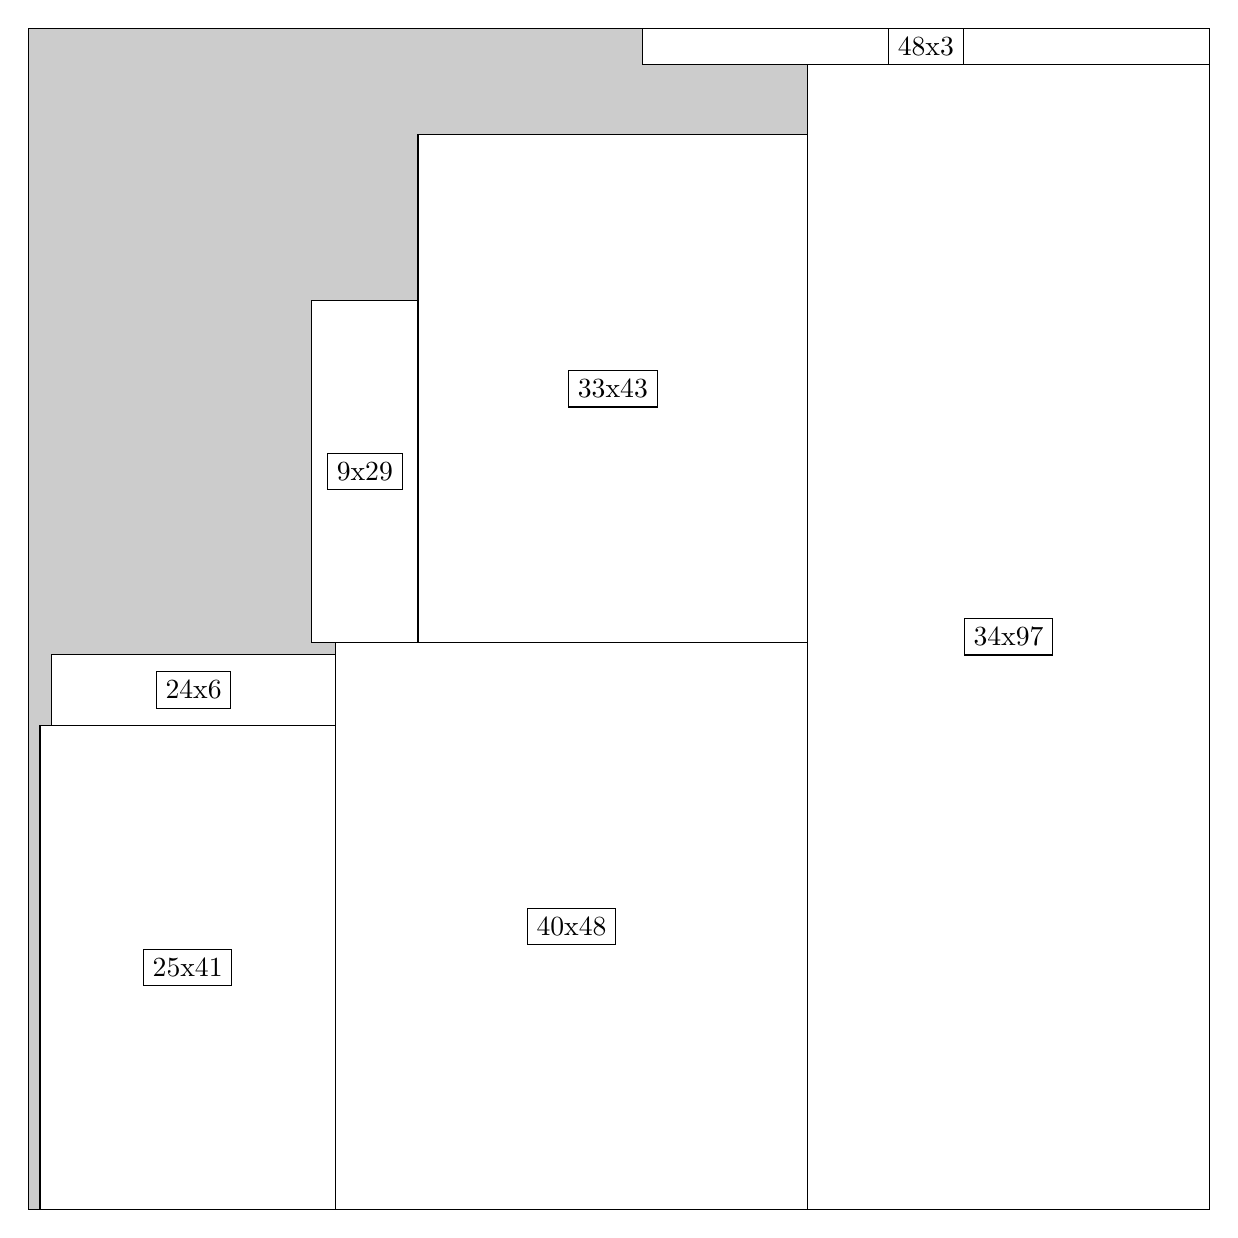
\begin{tikzpicture}[shorten >=1pt,scale=1.0,every node/.style={scale=1.0},->]
\tikzstyle{vertex}=[circle,fill=black!25,minimum size=14pt,inner sep=0pt]
\filldraw[fill=gray!40!white, draw=black] (0,0) rectangle (15.0,15.0);
\foreach \name/\x/\y/\w/\h in {34x97/9.9/0.0/5.1/14.549999999999999,40x48/3.9/0.0/6.0/7.199999999999999,25x41/0.15/0.0/3.75/6.1499999999999995,24x6/0.3/6.1499999999999995/3.5999999999999996/0.8999999999999999,33x43/4.95/7.199999999999999/4.95/6.45,9x29/3.5999999999999996/7.199999999999999/1.3499999999999999/4.35,48x3/7.8/14.549999999999999/7.199999999999999/0.44999999999999996}
\filldraw[fill=white!40!white, draw=black] (\x,\y) rectangle node[draw] (\name) {\name} ++(\w,\h);
\end{tikzpicture}


w =34 , h =97 , x =66 , y =0 , v =3298
\par
w =40 , h =48 , x =26 , y =0 , v =1920
\par
w =25 , h =41 , x =1 , y =0 , v =1025
\par
w =24 , h =6 , x =2 , y =41 , v =144
\par
w =33 , h =43 , x =33 , y =48 , v =1419
\par
w =9 , h =29 , x =24 , y =48 , v =261
\par
w =48 , h =3 , x =52 , y =97 , v =144
\par
\newpage


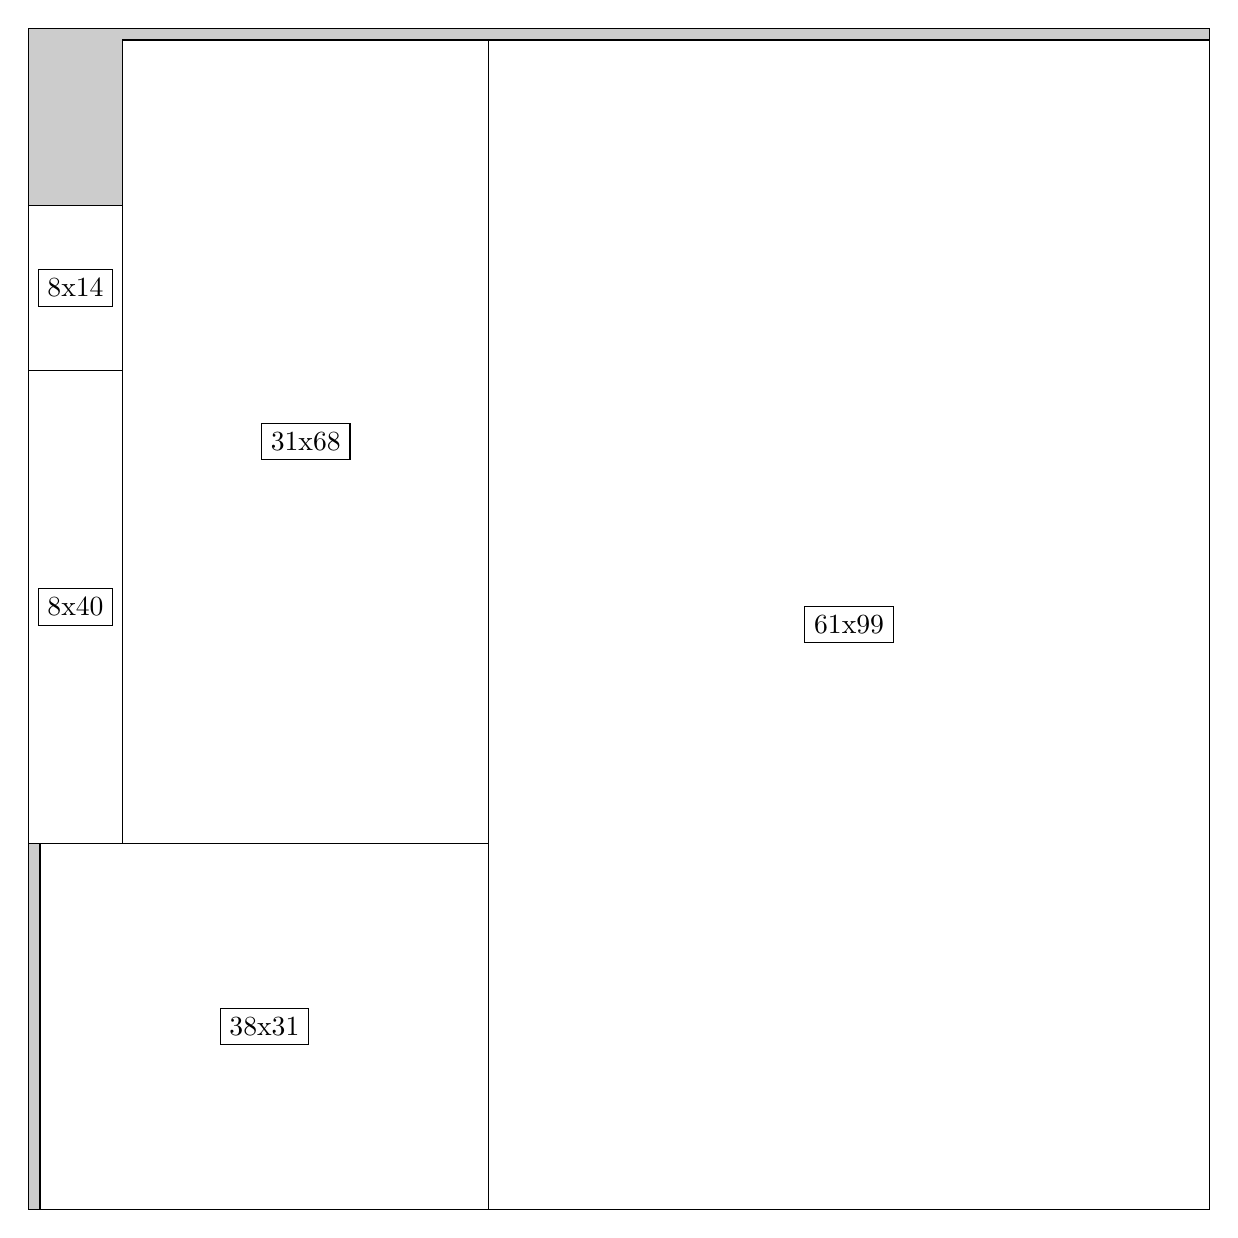
\begin{tikzpicture}[shorten >=1pt,scale=1.0,every node/.style={scale=1.0},->]
\tikzstyle{vertex}=[circle,fill=black!25,minimum size=14pt,inner sep=0pt]
\filldraw[fill=gray!40!white, draw=black] (0,0) rectangle (15.0,15.0);
\foreach \name/\x/\y/\w/\h in {61x99/5.85/0.0/9.15/14.85,38x31/0.15/0.0/5.7/4.6499999999999995,31x68/1.2/4.6499999999999995/4.6499999999999995/10.2,8x40/0.0/4.6499999999999995/1.2/6.0,8x14/0.0/10.65/1.2/2.1}
\filldraw[fill=white!40!white, draw=black] (\x,\y) rectangle node[draw] (\name) {\name} ++(\w,\h);
\end{tikzpicture}


w =61 , h =99 , x =39 , y =0 , v =6039
\par
w =38 , h =31 , x =1 , y =0 , v =1178
\par
w =31 , h =68 , x =8 , y =31 , v =2108
\par
w =8 , h =40 , x =0 , y =31 , v =320
\par
w =8 , h =14 , x =0 , y =71 , v =112
\par
\newpage


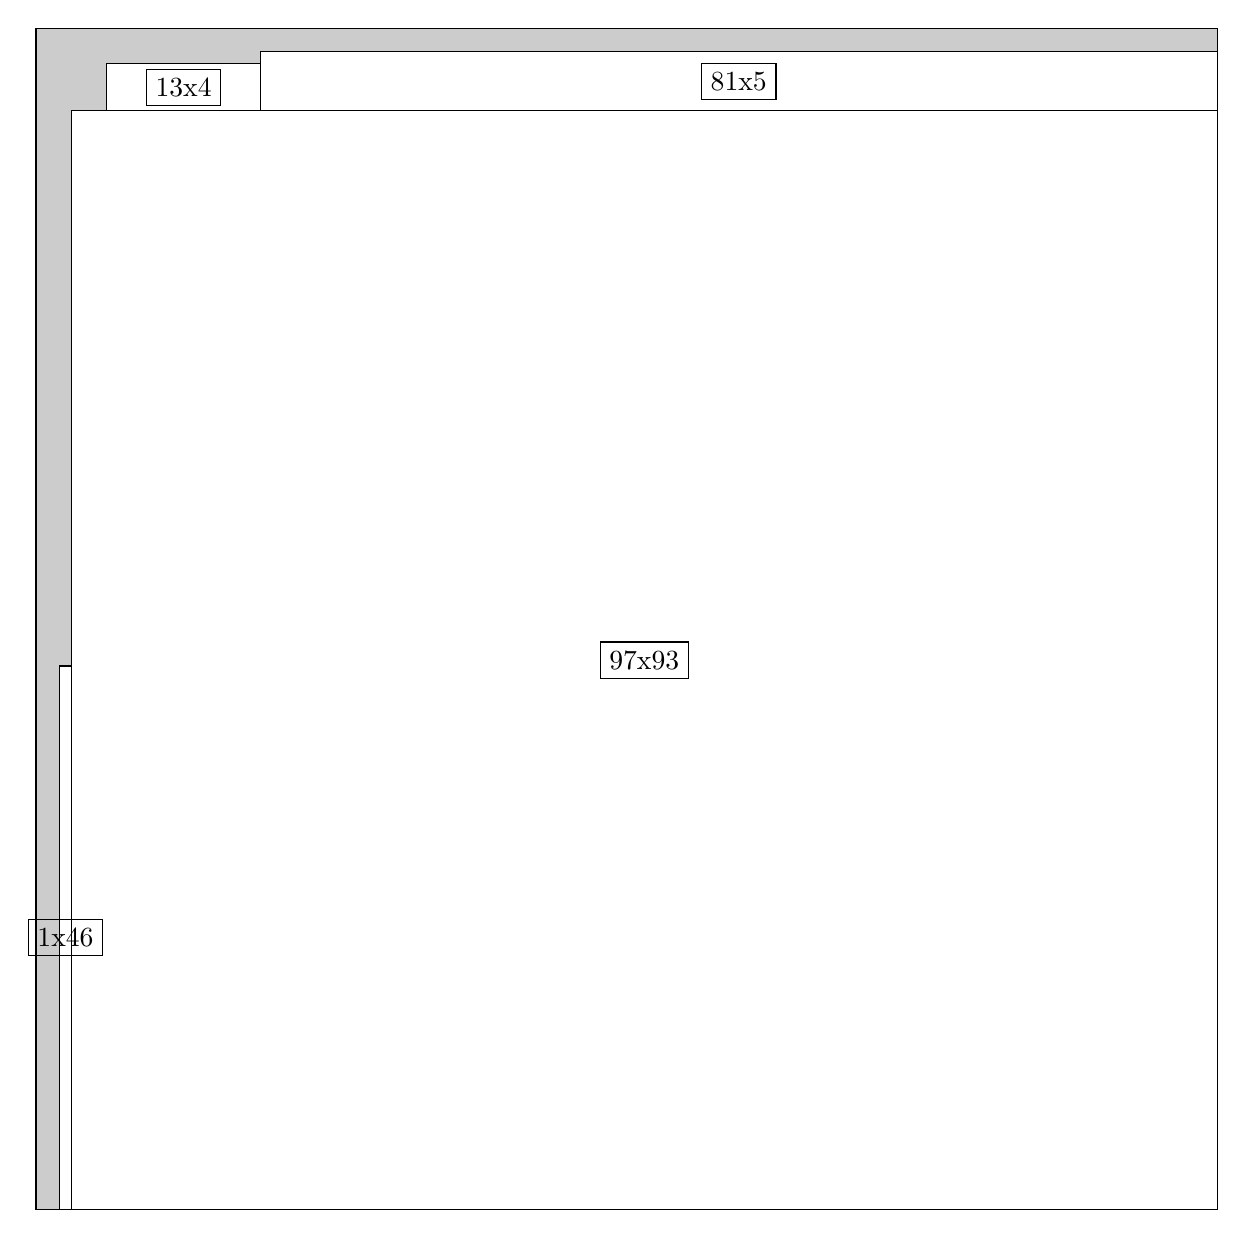
\begin{tikzpicture}[shorten >=1pt,scale=1.0,every node/.style={scale=1.0},->]
\tikzstyle{vertex}=[circle,fill=black!25,minimum size=14pt,inner sep=0pt]
\filldraw[fill=gray!40!white, draw=black] (0,0) rectangle (15.0,15.0);
\foreach \name/\x/\y/\w/\h in {97x93/0.44999999999999996/0.0/14.549999999999999/13.95,1x46/0.3/0.0/0.15/6.8999999999999995,81x5/2.85/13.95/12.15/0.75,13x4/0.8999999999999999/13.95/1.95/0.6}
\filldraw[fill=white!40!white, draw=black] (\x,\y) rectangle node[draw] (\name) {\name} ++(\w,\h);
\end{tikzpicture}


w =97 , h =93 , x =3 , y =0 , v =9021
\par
w =1 , h =46 , x =2 , y =0 , v =46
\par
w =81 , h =5 , x =19 , y =93 , v =405
\par
w =13 , h =4 , x =6 , y =93 , v =52
\par
\newpage


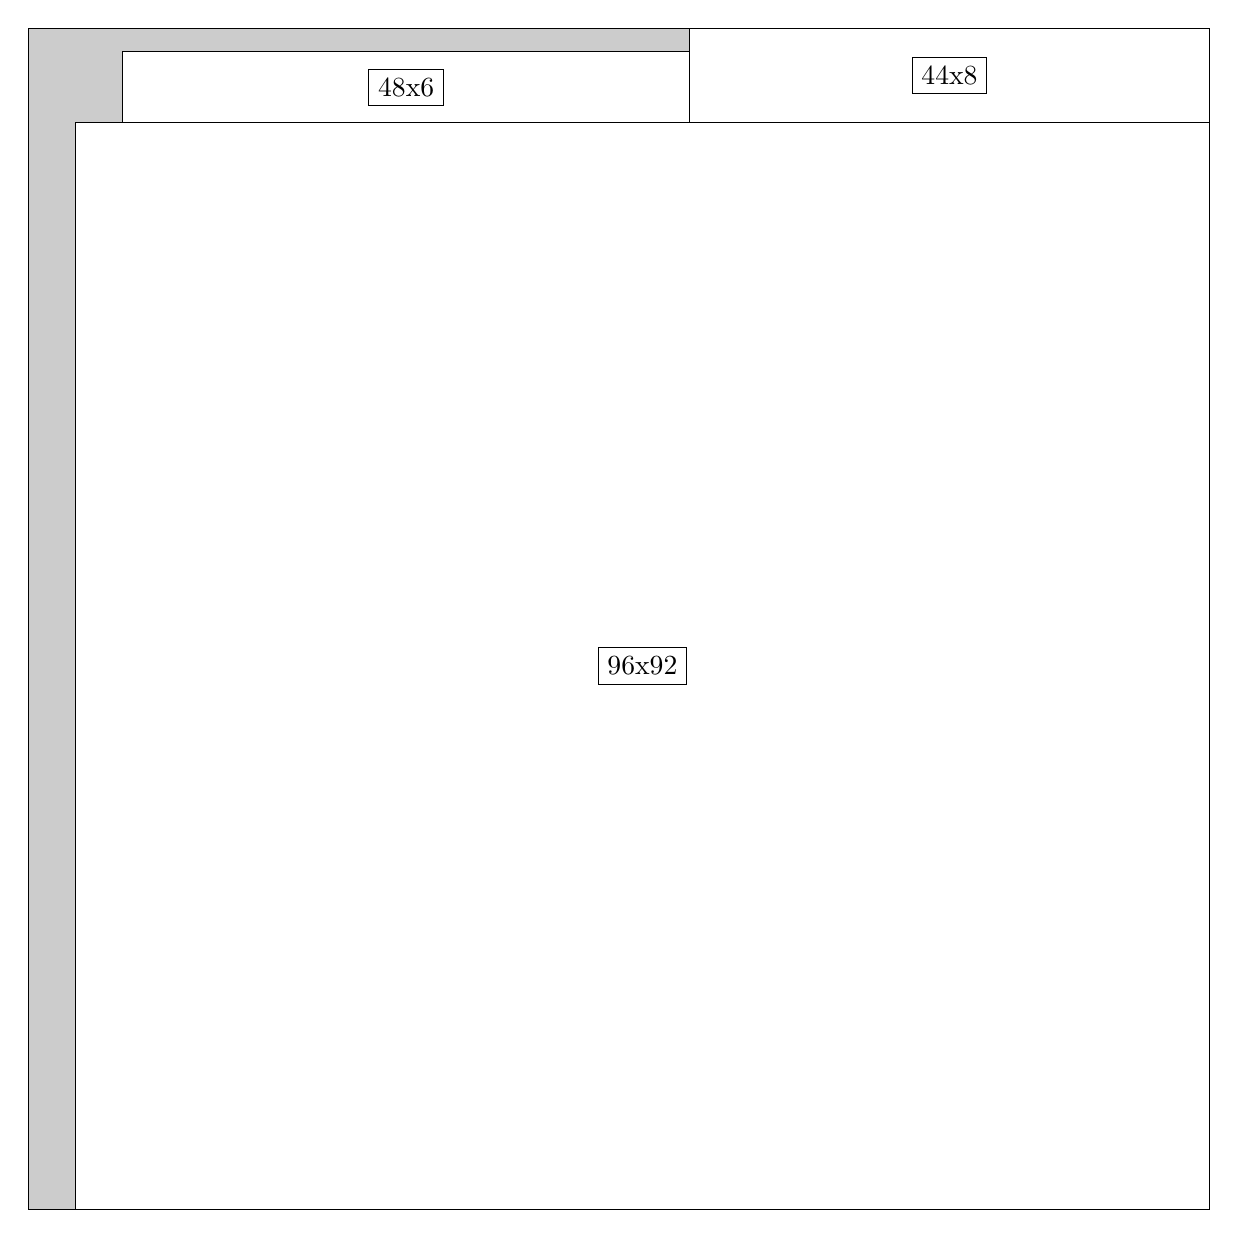
\begin{tikzpicture}[shorten >=1pt,scale=1.0,every node/.style={scale=1.0},->]
\tikzstyle{vertex}=[circle,fill=black!25,minimum size=14pt,inner sep=0pt]
\filldraw[fill=gray!40!white, draw=black] (0,0) rectangle (15.0,15.0);
\foreach \name/\x/\y/\w/\h in {96x92/0.6/0.0/14.399999999999999/13.799999999999999,44x8/8.4/13.799999999999999/6.6/1.2,48x6/1.2/13.799999999999999/7.199999999999999/0.8999999999999999}
\filldraw[fill=white!40!white, draw=black] (\x,\y) rectangle node[draw] (\name) {\name} ++(\w,\h);
\end{tikzpicture}


w =96 , h =92 , x =4 , y =0 , v =8832
\par
w =44 , h =8 , x =56 , y =92 , v =352
\par
w =48 , h =6 , x =8 , y =92 , v =288
\par
\newpage


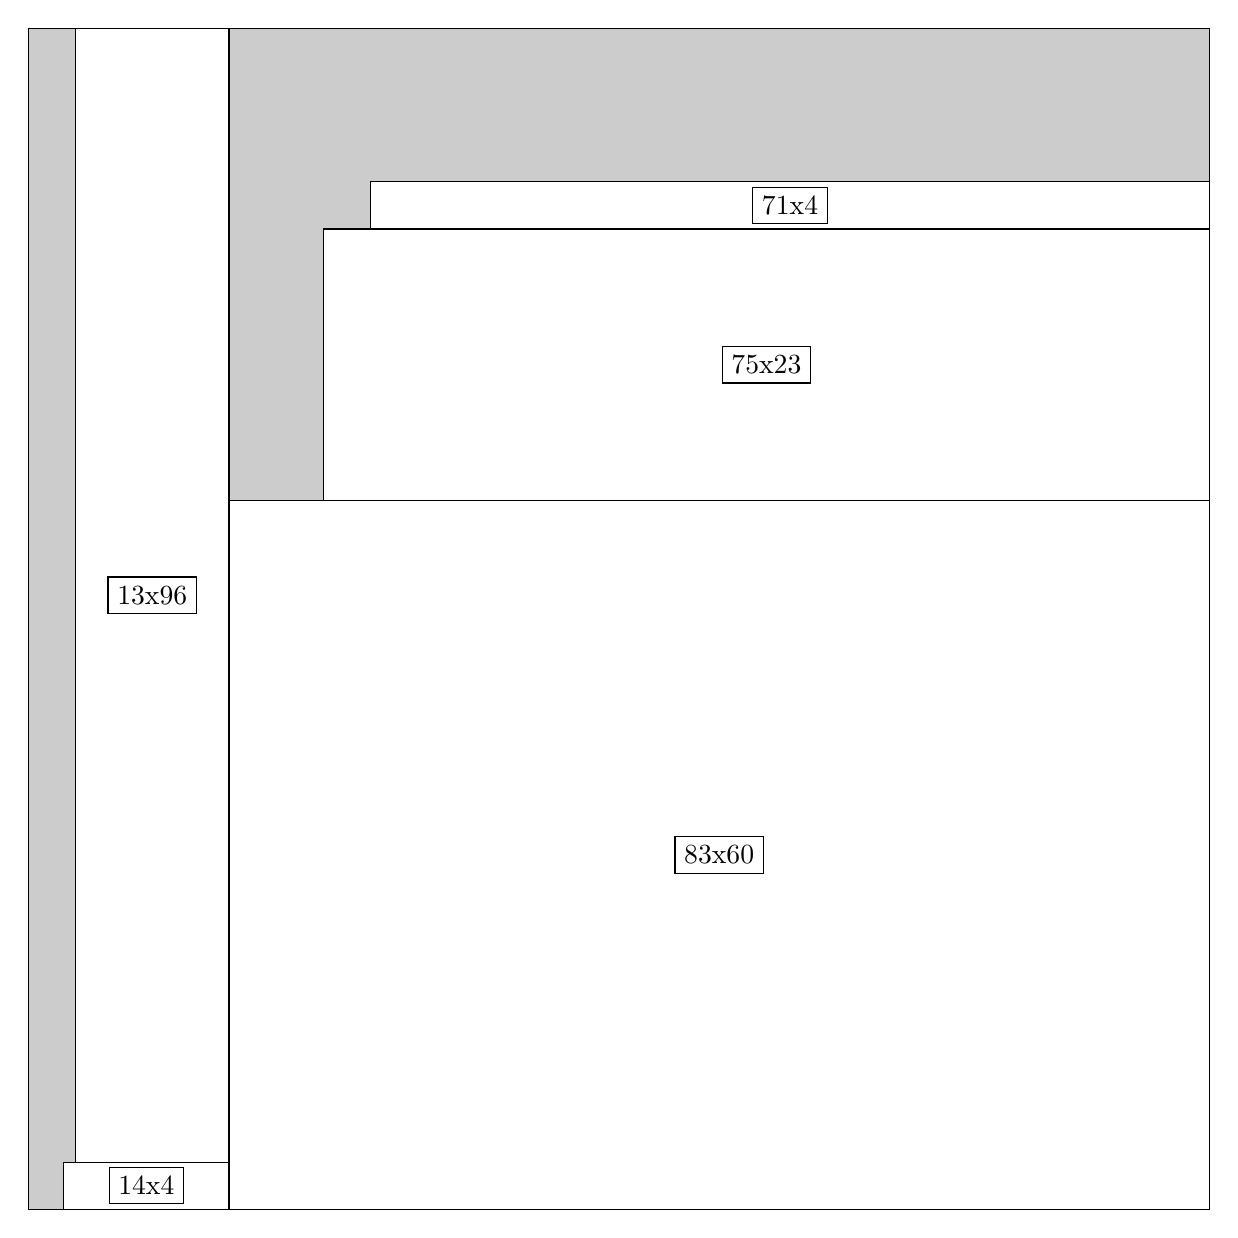
\begin{tikzpicture}[shorten >=1pt,scale=1.0,every node/.style={scale=1.0},->]
\tikzstyle{vertex}=[circle,fill=black!25,minimum size=14pt,inner sep=0pt]
\filldraw[fill=gray!40!white, draw=black] (0,0) rectangle (15.0,15.0);
\foreach \name/\x/\y/\w/\h in {83x60/2.55/0.0/12.45/9.0,75x23/3.75/9.0/11.25/3.4499999999999997,71x4/4.35/12.45/10.65/0.6,14x4/0.44999999999999996/0.0/2.1/0.6,13x96/0.6/0.6/1.95/14.399999999999999}
\filldraw[fill=white!40!white, draw=black] (\x,\y) rectangle node[draw] (\name) {\name} ++(\w,\h);
\end{tikzpicture}


w =83 , h =60 , x =17 , y =0 , v =4980
\par
w =75 , h =23 , x =25 , y =60 , v =1725
\par
w =71 , h =4 , x =29 , y =83 , v =284
\par
w =14 , h =4 , x =3 , y =0 , v =56
\par
w =13 , h =96 , x =4 , y =4 , v =1248
\par
\newpage


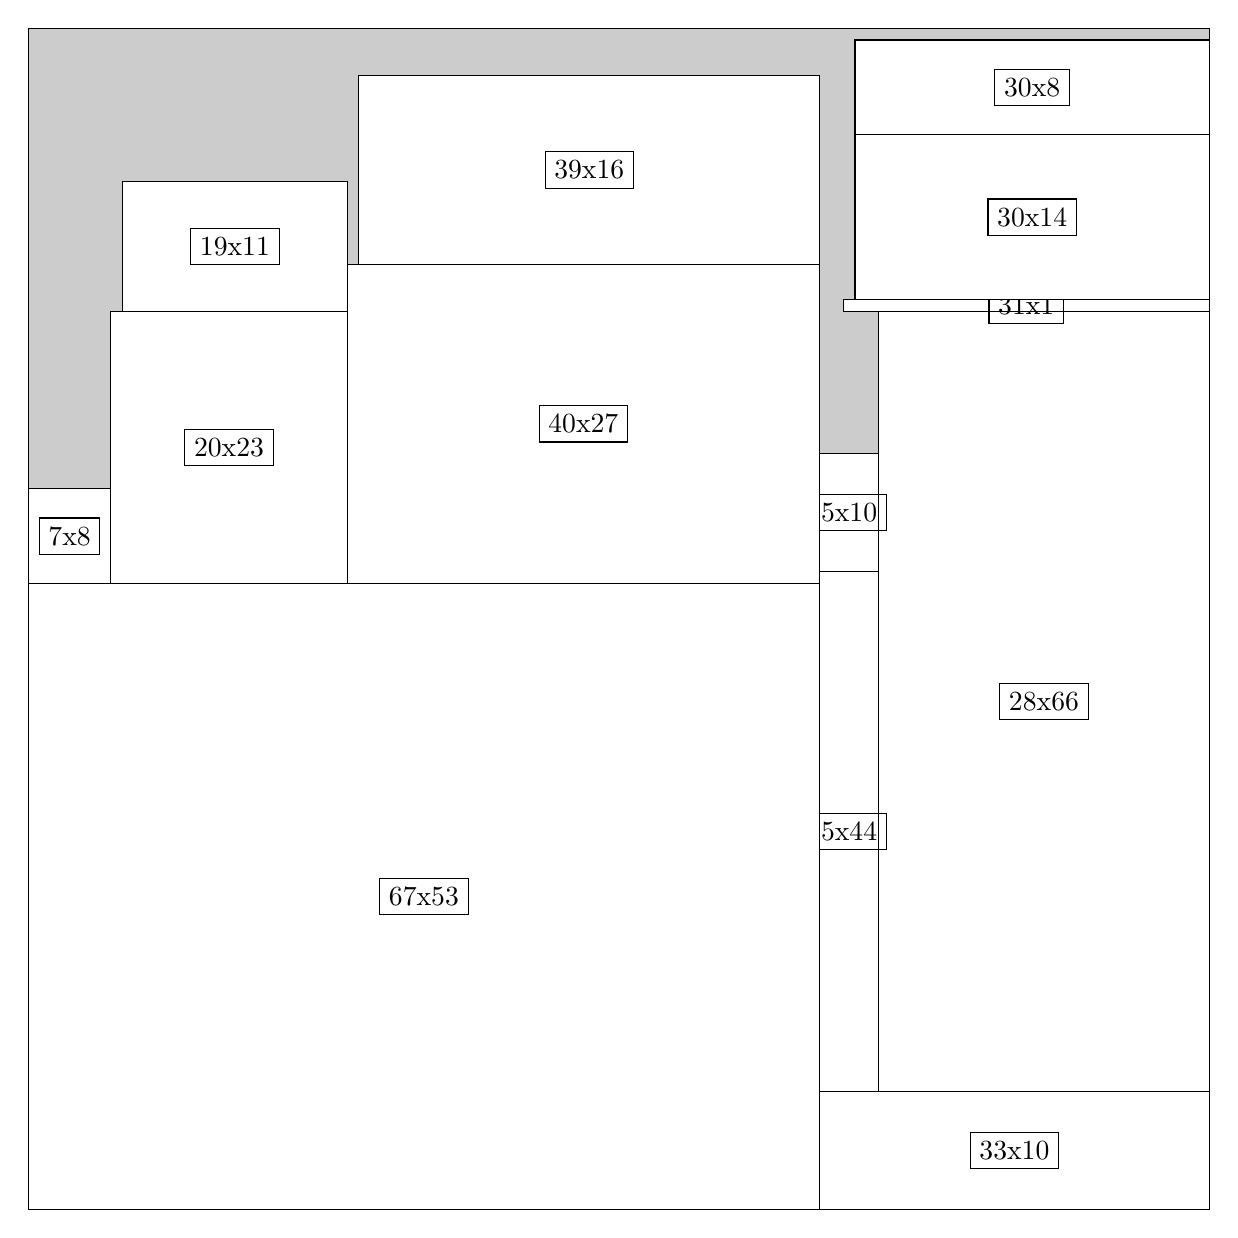
\begin{tikzpicture}[shorten >=1pt,scale=1.0,every node/.style={scale=1.0},->]
\tikzstyle{vertex}=[circle,fill=black!25,minimum size=14pt,inner sep=0pt]
\filldraw[fill=gray!40!white, draw=black] (0,0) rectangle (15.0,15.0);
\foreach \name/\x/\y/\w/\h in {33x10/10.049999999999999/0.0/4.95/1.5,28x66/10.799999999999999/1.5/4.2/9.9,5x44/10.049999999999999/1.5/0.75/6.6,5x10/10.049999999999999/8.1/0.75/1.5,31x1/10.35/11.4/4.6499999999999995/0.15,30x14/10.5/11.549999999999999/4.5/2.1,30x8/10.5/13.65/4.5/1.2,67x53/0.0/0.0/10.049999999999999/7.949999999999999,40x27/4.05/7.949999999999999/6.0/4.05,39x16/4.2/12.0/5.85/2.4,20x23/1.05/7.949999999999999/3.0/3.4499999999999997,7x8/0.0/7.949999999999999/1.05/1.2,19x11/1.2/11.4/2.85/1.65}
\filldraw[fill=white!40!white, draw=black] (\x,\y) rectangle node[draw] (\name) {\name} ++(\w,\h);
\end{tikzpicture}


w =33 , h =10 , x =67 , y =0 , v =330
\par
w =28 , h =66 , x =72 , y =10 , v =1848
\par
w =5 , h =44 , x =67 , y =10 , v =220
\par
w =5 , h =10 , x =67 , y =54 , v =50
\par
w =31 , h =1 , x =69 , y =76 , v =31
\par
w =30 , h =14 , x =70 , y =77 , v =420
\par
w =30 , h =8 , x =70 , y =91 , v =240
\par
w =67 , h =53 , x =0 , y =0 , v =3551
\par
w =40 , h =27 , x =27 , y =53 , v =1080
\par
w =39 , h =16 , x =28 , y =80 , v =624
\par
w =20 , h =23 , x =7 , y =53 , v =460
\par
w =7 , h =8 , x =0 , y =53 , v =56
\par
w =19 , h =11 , x =8 , y =76 , v =209
\par
\newpage


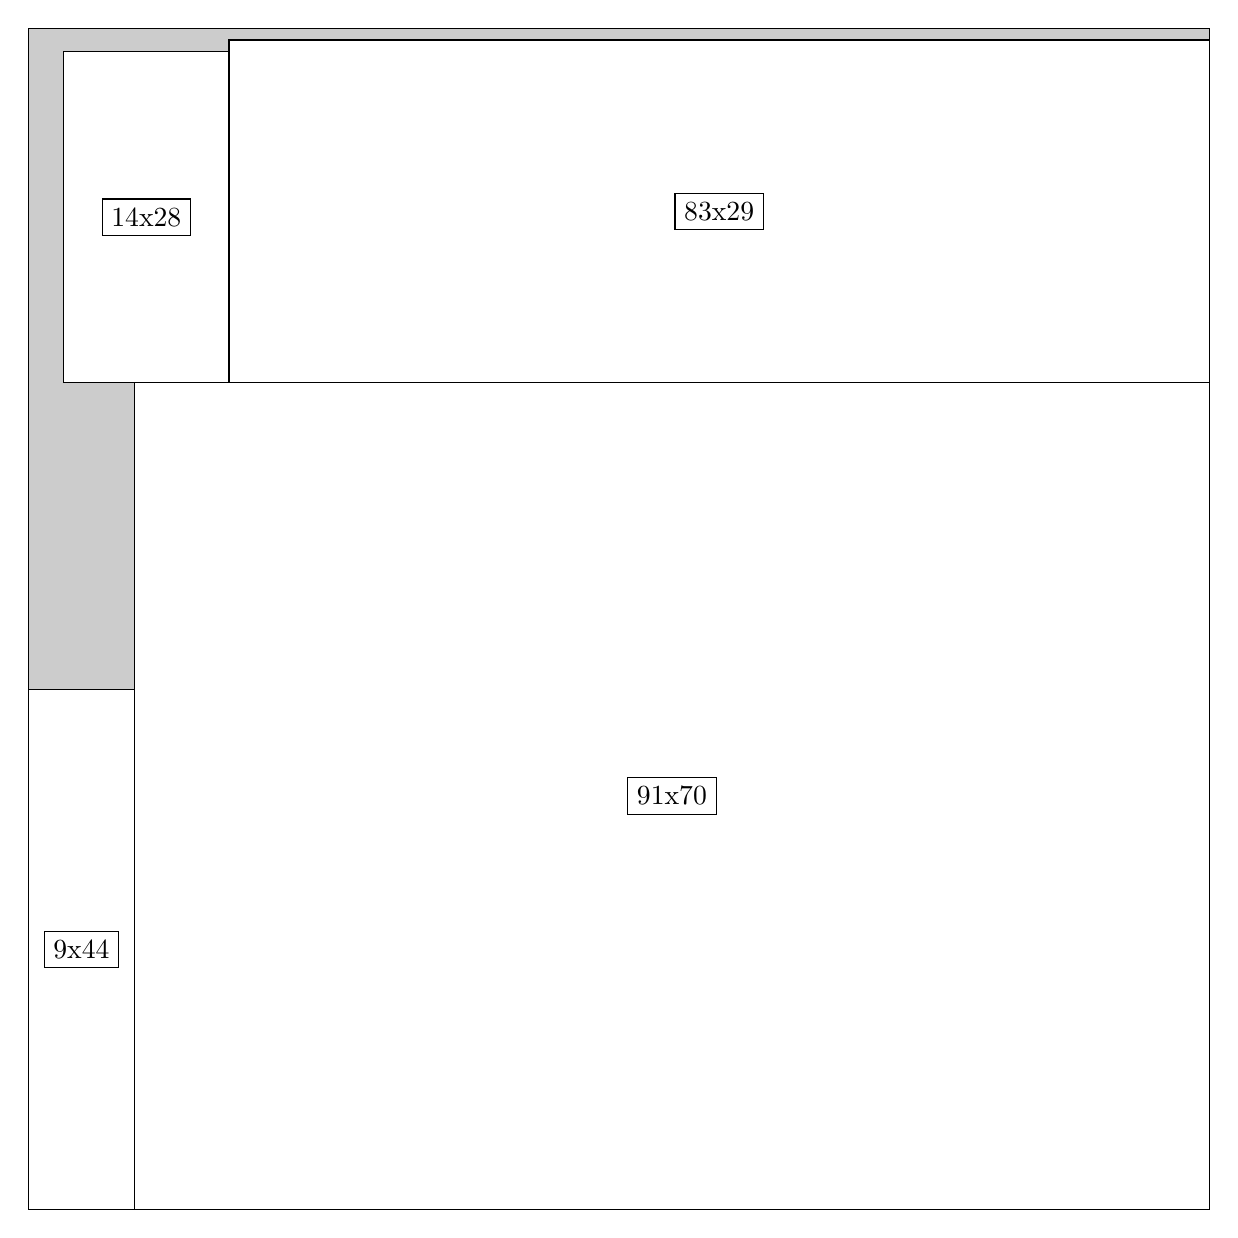
\begin{tikzpicture}[shorten >=1pt,scale=1.0,every node/.style={scale=1.0},->]
\tikzstyle{vertex}=[circle,fill=black!25,minimum size=14pt,inner sep=0pt]
\filldraw[fill=gray!40!white, draw=black] (0,0) rectangle (15.0,15.0);
\foreach \name/\x/\y/\w/\h in {91x70/1.3499999999999999/0.0/13.65/10.5,9x44/0.0/0.0/1.3499999999999999/6.6,83x29/2.55/10.5/12.45/4.35,14x28/0.44999999999999996/10.5/2.1/4.2}
\filldraw[fill=white!40!white, draw=black] (\x,\y) rectangle node[draw] (\name) {\name} ++(\w,\h);
\end{tikzpicture}


w =91 , h =70 , x =9 , y =0 , v =6370
\par
w =9 , h =44 , x =0 , y =0 , v =396
\par
w =83 , h =29 , x =17 , y =70 , v =2407
\par
w =14 , h =28 , x =3 , y =70 , v =392
\par
\newpage


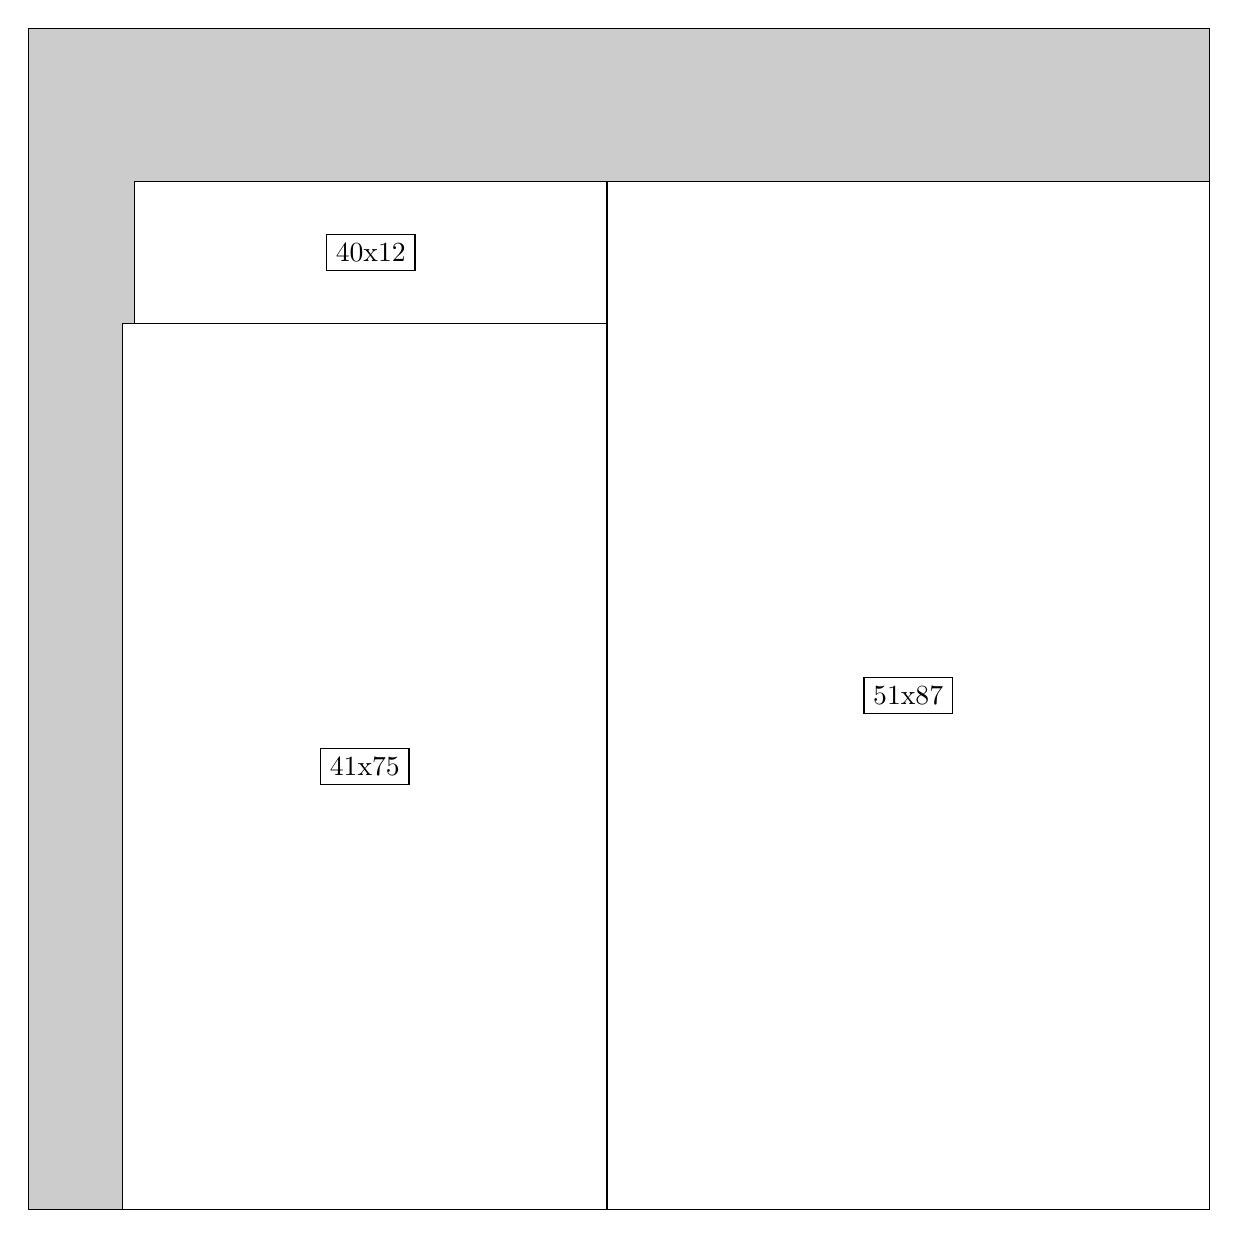
\begin{tikzpicture}[shorten >=1pt,scale=1.0,every node/.style={scale=1.0},->]
\tikzstyle{vertex}=[circle,fill=black!25,minimum size=14pt,inner sep=0pt]
\filldraw[fill=gray!40!white, draw=black] (0,0) rectangle (15.0,15.0);
\foreach \name/\x/\y/\w/\h in {51x87/7.35/0.0/7.6499999999999995/13.049999999999999,41x75/1.2/0.0/6.1499999999999995/11.25,40x12/1.3499999999999999/11.25/6.0/1.7999999999999998}
\filldraw[fill=white!40!white, draw=black] (\x,\y) rectangle node[draw] (\name) {\name} ++(\w,\h);
\end{tikzpicture}


w =51 , h =87 , x =49 , y =0 , v =4437
\par
w =41 , h =75 , x =8 , y =0 , v =3075
\par
w =40 , h =12 , x =9 , y =75 , v =480
\par
\newpage


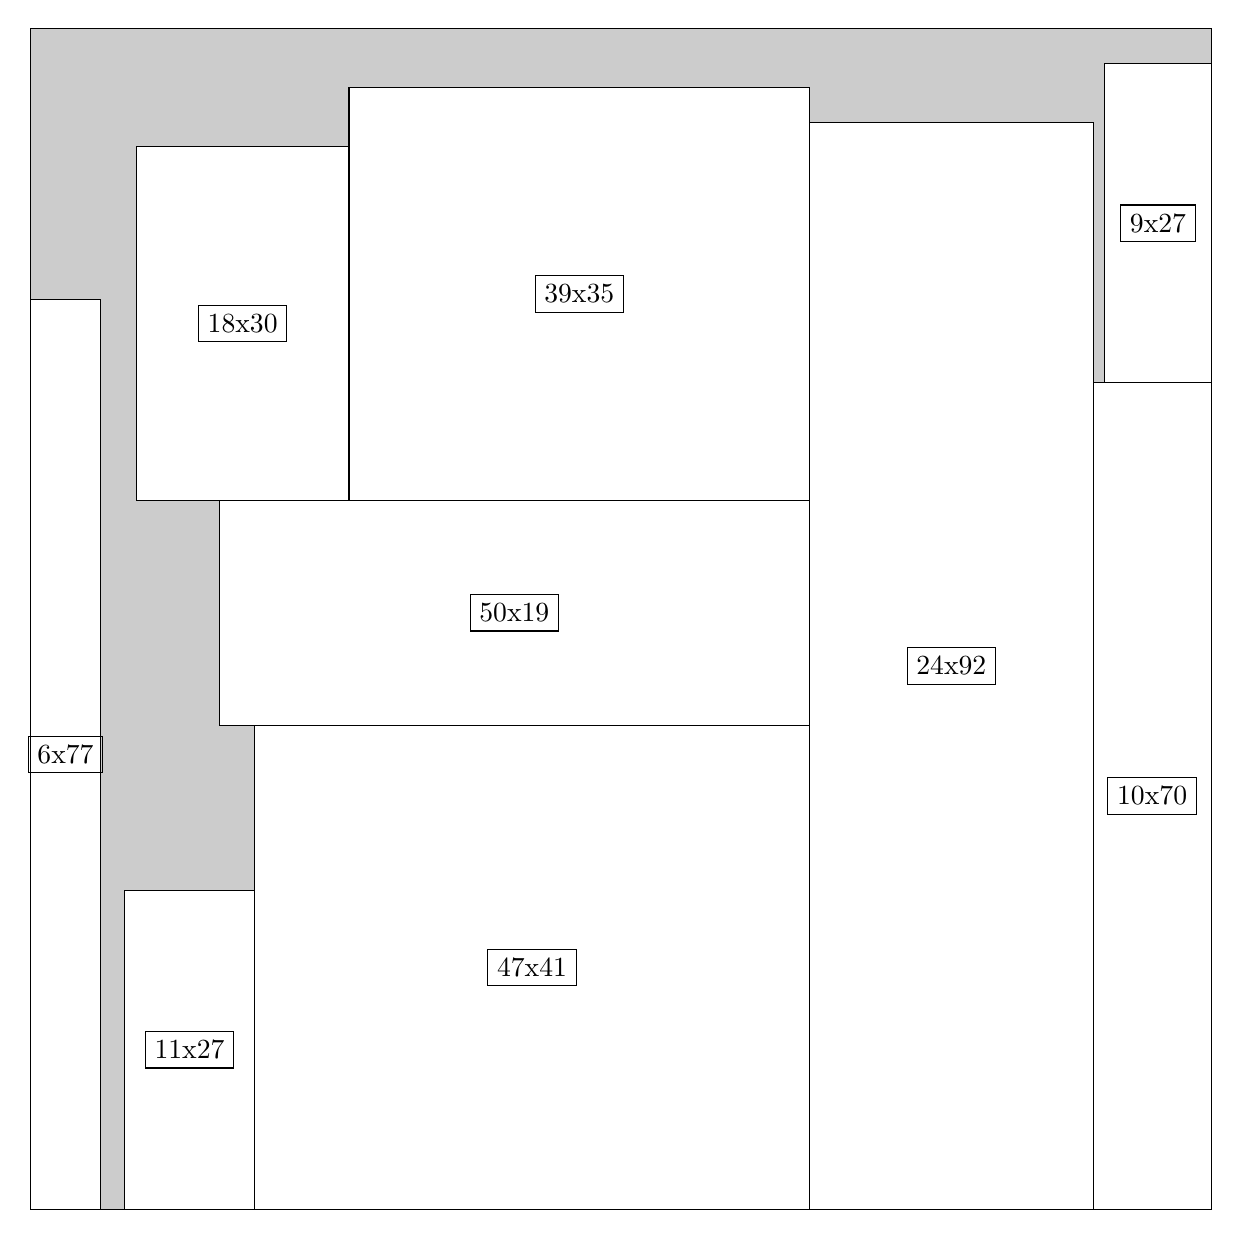
\begin{tikzpicture}[shorten >=1pt,scale=1.0,every node/.style={scale=1.0},->]
\tikzstyle{vertex}=[circle,fill=black!25,minimum size=14pt,inner sep=0pt]
\filldraw[fill=gray!40!white, draw=black] (0,0) rectangle (15.0,15.0);
\foreach \name/\x/\y/\w/\h in {10x70/13.5/0.0/1.5/10.5,9x27/13.65/10.5/1.3499999999999999/4.05,24x92/9.9/0.0/3.5999999999999996/13.799999999999999,47x41/2.85/0.0/7.05/6.1499999999999995,11x27/1.2/0.0/1.65/4.05,50x19/2.4/6.1499999999999995/7.5/2.85,39x35/4.05/9.0/5.85/5.25,18x30/1.3499999999999999/9.0/2.6999999999999997/4.5,6x77/0.0/0.0/0.8999999999999999/11.549999999999999}
\filldraw[fill=white!40!white, draw=black] (\x,\y) rectangle node[draw] (\name) {\name} ++(\w,\h);
\end{tikzpicture}


w =10 , h =70 , x =90 , y =0 , v =700
\par
w =9 , h =27 , x =91 , y =70 , v =243
\par
w =24 , h =92 , x =66 , y =0 , v =2208
\par
w =47 , h =41 , x =19 , y =0 , v =1927
\par
w =11 , h =27 , x =8 , y =0 , v =297
\par
w =50 , h =19 , x =16 , y =41 , v =950
\par
w =39 , h =35 , x =27 , y =60 , v =1365
\par
w =18 , h =30 , x =9 , y =60 , v =540
\par
w =6 , h =77 , x =0 , y =0 , v =462
\par
\newpage


\end{document}